\documentclass[12pt]{article}
\usepackage{url, graphicx}
\usepackage{geometry}
\usepackage{amsmath}
 \geometry{
 a4paper,
 total={170mm,257mm},
 left=20mm,
 top=20mm,
 }

\title{\huge Lecture 1}
\author{Yutong Yan}
\date{}

\begin{document}
\maketitle

\section{The Central Paradigm of Computer Science}
\renewcommand{\labelitemii}{$\circ$}
\renewcommand{\labelitemiii}{$\cdot$}
\begin{itemize}
\item The central \textbf{\textit{paradigm}}  in computer science is that an algorithm \textbf{\textit{A}} is good if:
	\begin{itemize}
	\item \textbf{\textit{A}} runs in \textbf{\textit{polynomial time}} in the input size n.
	\item That is, \textbf{\textit{A}} runs in time $T$(n) = $O$($n^k$) for some constant number k.
		\begin{itemize}
		\item $T$(n) = 100n + 55
		\item $T$(n) = \( \frac{1}{2} \)$n^2$ + $999\log{}n$
		\item $T$(n) = 6$n^7$ + 900000$n^2$ - $\sqrt{n}$			
		\end{itemize}
	\item An algorithm is \textbf{\textit{bad}} if it runs in exponential time.
		\begin{itemize}
		\item $T$(n) = $2^n$ + 100$n^5$
		\item $T$(n) = $1.000000001^n$ - $n^3$ - n 
		\end{itemize}	
	\item An algorithm is \textbf{\textit{good}} if it runs in \textbf{\textit{polynomial time}} in the input size n.
	\begin{center}
	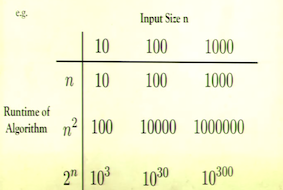
\includegraphics{lecture1a}
	\end{center}
	\end{itemize}
\end{itemize}


\section{Good versus Bad (Algorithms)}
\renewcommand{\labelitemii}{$\circ$}
\renewcommand{\labelitemiii}{$\cdot$}
\begin{itemize}
\item For example, consider the problem of sorting n numbers.
	\begin{itemize}
	\item A Good Algorithm: \textbf{MergeSort} runs in time $O$($n \cdot log{}n$)
	\item A Bad Algorithm: \textbf{BruteForce Search} runs in time $O$($n \cdot n!$) \(\gg\) $2^n$
	\end{itemize}
\end{itemize}


\section{An Equivalent Characterization}
\renewcommand{\labelitemii}{$\circ$}
\renewcommand{\labelitemiii}{$\cdot$}
\renewcommand{\labelitemiii}{$\rightarrow$}
\begin{itemize}
\item This central \textbf{\textit{paradigm}} has an equivalent formulation
	\begin{itemize}
	\item \textbf{\textit{A}} runs in \textbf{\textit{polynomial time}} in the input size n.
	\item The input sizes that \textbf{\textit{A}} can solve, in a fixed amount $T$ of time, \textbf{\textit{scales multiplicatively}} with increasing computational power.
	\begin{center}
	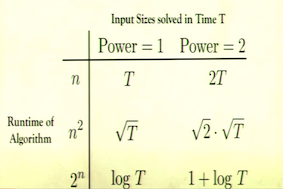
\includegraphics{lecture1b}
	\bigbreak
	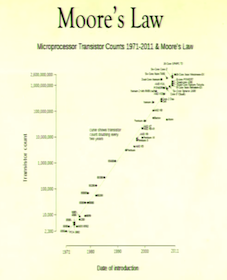
\includegraphics{lecture1c}
	\end{center}
	\item Moore's Law: Computational power \textit{doubles} roughly every two years.
		\begin{itemize}
		\item Functional time algorithms will never be able to solve large problems.
		\end{itemize}
	\end{itemize}

\clearpage	
\item The practical implications are perhaps simpler to understand with this \underline{latter} formulation.
\item Thus, improvements in hardware will \textit{never} overcome \textbf{\textit{bad algorithm design}}.
\item Indeed, the current dramatic breakthroughs in computer science are based upon batter (faster and higher performance) algorithmic techniques.
\end{itemize}


\section{Robustness}
\renewcommand{\labelitemii}{$\circ$}
\renewcommand{\labelitemiii}{$\cdot$}
\renewcommand{\labelitemiii}{$\rightarrow$}
\begin{itemize}
\item This measure of quality or "goodness" is \textbf{\textit{robust}}
	\begin{center}
	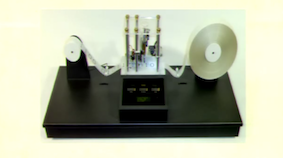
\includegraphics{lecture1d}
	\end{center}
\item All reasonable models of algorithms are polynomial time equivalent.
	\begin{itemize}
	\item Otherwise one model could perform, say, an exponential number of operations in the time another model took to perform just one.
	\end{itemize}
\item The standard formal model is the \textbf{Turing Machine}.
\end{itemize}
\section{Cryptography (Just an example of the course)}
\renewcommand{\labelitemii}{$\circ$}
\renewcommand{\labelitemiii}{$\cdot$}
\renewcommand{\labelitemiii}{$\rightarrow$}
\begin{itemize}
\item Alice wants to send Bob a message.\\
\noindent But she is worried that Eve might intercept the message.\\
\noindent She decides to encrypt the message $M$ as $\hat{M} = f(M)$.\\
\noindent Bob can then decrypt the message via $f^{-1}$($\hat{M}$) = $f^{-1}$($f$($M$)) = $M$\\
\noindent Eve cannot understand the message.\\
\noindent Alice encrypts the message $M$ with the (encryption) lock $f$.\\
\noindent Bob decrypts the message $\hat{M}$ with the (decryption) key $f^{-1}$.\\
\noindent Because Eve does not have the key she cannot decipher the message.\\
\noindent Two major problems occur.
\item Problem one:
	\begin{itemize}
	\item Eve might be able to break the code.
		\begin{itemize}
		\item That is , given $\hat{M}$ she may be able to reconstruct $f$ and then $f^{-1}$.
		\end{itemize}
	\item Standard techniques for code-breaking include:
		\begin{itemize}
		\item Frequency Analysis
			\begin{itemize}
			\item $e.g.$ "e" is the most common letter and "the" is the most common word in 					English.
			\end{itemize}
		\item Cribs. 
			\begin{itemize}
			\item $e.g.$ German weather reports were exploited to help decode messages 						from 	the "unbreakable" \textbf{Enigma Machine}.
			\end{itemize}
		\end{itemize}
	\end{itemize}

\item Problem Two:
	\begin{itemize}
	\item Alice and Bob need to agree on what the encryption code (lock) $f$ is.
	\item But to do this they need to exchange a message discussing the code.
	\end{itemize}
\item Public-Key Cryptography
	\begin{itemize}
	\item In face, Bob gives absolutely everyone a copy of the (encryption) lock.
	\item Everyone can send the message and Bob has the key.
	\item The lock is made public. This is called public-key cryptography.
	\item But this idea sounds completely crazy.
		\begin{itemize}
		\item Doesn't this solution to Problem Two make Problem One inevitable?
		\item That is, if Eve has the lock $f$ then won't she use it to decode $f(M)$?
		\end{itemize}
	\item No, not if $f$ is hard to invert for anybody except Bob himself.
	\item But do such functions $f$ that are hard to invert \textbf{exist}?
	\item Yes!
	\end{itemize}
\item RSA Encryption
	\begin{enumerate}
	\item Bob chooses two large prime numbers $q_{1}$, $q_{2}$ and a large number $p$ that is co-prime to ($q_{1}$ - 1) $\cdot$ ($q_{2}$ - 1)
	\item Bob's public key is ($p$, $n$) where $n$ = $q_{1}$ $\cdot$ $q_{2}$ 
	
		\hspace*{\fill}Encryption: $\hat{M}$ = $M^p$ mod n\hspace*{\fill}
		
	\item Bob's prime key is ($q_1$, $q_2$, x) where x is the inverse of p modular ($q_{1}$ - 1) $\cdot$ ($q_{2}$ - 1)
	
		\hspace*{\fill}Decryption: $M$ = $\hat{M}^x$ mod n\hspace*{\fill}
		
		\begin{itemize}
		\item p = $2^{16}$ + 1
		\item $q_1$, $q_2$ = 2048 bits
		\end{itemize}
	\item An Example
		\begin{enumerate}
		\item Prime numbers $q_1$, $q_2$ and number p co-prime to ($q_{1}$ - 1) $\cdot$ 				($q_{2}$ - 1) \\
		\noindent p = 7, $q_1$ = 3, $q_2$ = 11 valid as gcd(7,20) = 1
		\item Public key (p,n) where n = $q_1$ $\cdot$ $q_2$\\
		\noindent n = 33
		\item Private Key ($q_1$, $q_2$, x) where x is the inverse of p mod ($q_{1}$ - 1) $\cdot$ 			($q_{2}$ - 1) \\
		\noindent x = 33 as 3 $\cdot$ 7 = 1 mod 20\\
		\noindent Public: n = 33, p = 7 \\
		\noindent Private $q_1$ = 3, $q_2$ = 11, x = 3\\
			\begin{center}
			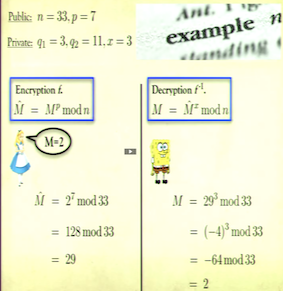
\includegraphics{lecture1e}
			\end{center}
		\end{enumerate}
	\end{enumerate}
\item Is RSA Encryption Safe?
	\begin{itemize}
	\item Public-key cryptography lies at the heart of the modern economy.
		\begin{itemize}
		\item Financial Services
		\item Online Shopping
		\item Secure Messaging
		\end{itemize}
	\item So it is extremely important that the method is safe.
	\item We claim it is because:
		\begin{itemize}
		\item Bob has a good  algorithm for decryption.
		\item Eve only has a bad algorithm for decryption.
		\end{itemize}
	\end{itemize}
\item Bob has a Good Decryption Algorithm
	\begin{itemize}
	\item Initially, Bob can do the following in polynomial time.
		\begin{itemize}
		\item Choose the primes $q_1$, $q_2$ 
		\item Choose a number p that is co-prime with ($q_{1}$ - 1) $\cdot$ 	($q_{2}$ - 1)
		\item Find x the inverse (Using Euclid's Algorithm) of p and ($q_{1}$ - 1) $\cdot$ ($q_{2}$ 			- 1)
		\end{itemize}
	\item Using fast exponentiation, encoding and decoding is polynomial time.
	
	\hspace*{\fill}Encryption: $\hat{M}$ = $M^p$ mod n\hspace*{\fill}
		
	\end{itemize}
\item Eve has a Bad Decryption Algorithm

	\hspace*{\fill}Decryption: $M$ = $\hat{M}^x$ mod n\hspace*{\fill}
		
	\begin{itemize}
	\item To decrypt Eve needs to find x the inverse of p and ($q_{1}$ - 1) $\cdot$ ($q_{2}$ 			- 1)
		\begin{itemize}
		\item She knows p, but does not know $q_1$, $q_2$
		\item Instead, she only knows n = $q_1$ $\cdot$ $q_2$
		\end{itemize}
	\item So to find $q_1$, $q_2$, she needs to find the prime factorization of n.
	\item But it is believed that finding the prime factors of a b-bit number is hard.
		\begin{itemize}
		\item Instead, the obvious algorithm attempts to divide n by each integer in the range 			\{2,3, ... ,$2^b$\} $\leftarrow$ 4096 bits
		\end{itemize}
	\item In fact, if 	Eve could find x without $q_1$, $q_2$, then she could use x to find $q_1$, 		$q_2$. That is, she could factor n.\\
	\noindent $\Rightarrow$ Eve only has exponential time algorithm to decrypt.
	\end{itemize}
\end{itemize}




























\end{document}